\chapter[Ferramentas de Gestão de Requisitos]{Ferramentas de Gestão de Requisitos}
Nesta seção do documento serão discutidas três ferramentas para gestão de requisitos e analisadas para que seja escolhida uma, entre elas, que se adeque melhor ao nosso processo de Engenharia de Requisitos utilizado no nosso contexto de negócio, Empresa Júnior de Engenharia de Energia da Universidade de Brasília.

\section[Ferramentas encontradas]{Ferramentas encontradas}

\subsection{Tiger Pro}
O Tiger Pro (Tool to InGest and Elucidate Requirements PROfessional) é uma ferramenta de gerenciamento de requisitos licenciada para o uso educacional que permite que os requisitos, além de também poderem ser adicionados diretamente no programa, possam ser adicionados através de documentos.

“Produz um sumário de informações na elucidação de requisitos, alocação de prioridades, definição de riscos e estimativa de custo em formato de texto ou gráfico.”[ANANIAS, 2009].

Apesar do software ser licenciado para o uso educacional, é possível utilizá-lo para fins comerciais, desde que haja uma autorização do responsável pelo software.

\subsection{TraceCloud}
TraceCloud é um software para gerência de requisitos independente se o projeto possui abordagem adaptativa ou se possui abordagem tradicional. Esse software gerencia as mudanças dos requisitos, desde mudanças de baixo nível até as de mais alto nível. Além disso, o TraceCloud dá um suporte completo de rastreabilidade dos requisitos.

O TraceCloud é bastante flexível ou seja, ele se adapta a qualquer processo de negócio. Vale ressaltar que dentro do contexto de nosso projeto, onde os atributos de requisitos foram outrora definidos, o TraceCloud fornece suporte a cada atributo.

O TraceCloud não é gratuito, mas possui versão gratuita para testes.

\subsection{Caliber}
O Caliber possui uma solução completa para gerenciamento de requisitos que garante a conformidade e alinhamento de desenvolvimento para atender as necessidades de negócios. Ele facilita a colaboração dos Stakeholders, possui uma visualização rica, gerenciamento robusto e uma rastreabilidade dos requisitos bem definida e completa.

O Caliber garante a entrega de um software com maior precisão e que atenda as necessidades dos clientes.

O software permite a participação do usuário de forma direta com o processo aumentando a clareza e precisão. Com isso, o usuário dá feedbacks para garantir que os requisitos não sejam definidos de forma inequívoca.

O Caliber fornece uma rastreabilidade completa dos requisitos para modelar as relações internas e externas dos mesmos.  Essa rastreabilidade suporta as mudanças dos requisitos  e responde como essas mudanças causam impacto no projeto.

O Caliber não é gratuito, mas possui versão de 30 dias para testes.

\section[Análise das Ferramentas]{Análise das Ferramentas}
Foram instaladas e testadas cada uma das ferramentas pesquisadas para que fosse decidido qual das três se adequasse melhor ao processo.

\subsection{Tiger Pro}
A instalação da ferramenta pode ser feita de maneira bem trivial, no entanto é necessária uma base de dados para que a ferramenta funcione. Essa necessidade pode ser suprida por meio do uso de um arquivo do tipo CSV ou utilizando uma base de dados MySQL ou Oracle, por exemplo.

A ferramenta tem quase 10 anos de lançamento, sem novas atualizações desde 2006. Possui interface um pouco confusa, mas aparentemente funcional. Dentre aos dados relacionadas com os requisitos, os mais importantes que a ferramenta permite o gerenciamento são:
\begin{itemize}
  \item Critérios de Aceitação;
  \item Análise Relacional ou Base Lógica;
  \item Rastreabilidade;
  \item Prioridade;
  \item Risco;
  \item Estimativa de Custos.
\end{itemize}

Dentre os atributos de requisitos que foram definidos para controlar e informar sobre os requisitos no projeto, apenas Prioridade foi encontrado na ferramenta.
A ferramenta permite o gerenciamento de outros atributos, porém estes outros não foram definidos previamente e nem observamos vantagens no seu uso para o projeto atual.
Por causa da limitação da ferramenta em relação aos atributos que ela controla e os atributos que escolhemos, e por ser uma ferramenta já descontinuada, a ferramenta não
se adequa ao processo definido.

\begin{figure}[!htb]
\centering
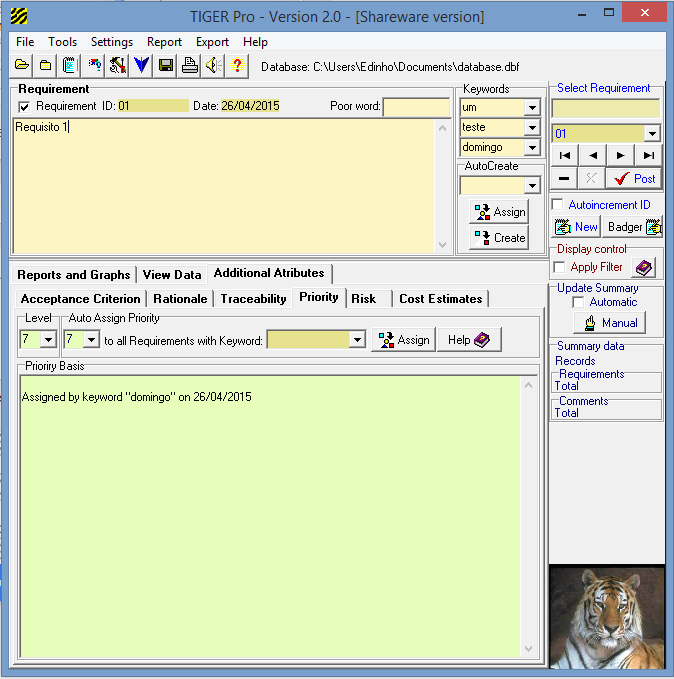
\includegraphics[scale=0.4]{figuras/tiger-pro.png}
\caption{Tela inicial da ferramenta Tiger-Pro}
\end{figure}

\begin{figure}[!htb]
\subsection{TraceCloud}
Não há grandes problemas no que se refere a instalação da ferramenta, pois ela é \textit{online}. A ferramenta pode ser usada por um grupo de usuários e os dados da mesma podem ser alterados por todos os envolvidos no projeto. Uma das grandes desvantagens da ferramenta, se refere ao fato da mesma ser via \textit{Web}, ou seja, em locais em que não há acesso a internet, é impossível de se trabalhar.

A ferramenta vai de encontro com o que o grupo definiu como atributos de estudo, pois ela registra perfeitamente e de forma intuitiva as características dos requisitos que são gerenciadas pela mesma, algumas delas são:
\begin{itemize}
  \item Gerência de mudanças;
  \item Status de aprovação dos requisitos;
  \item Status de andamento das atividades envolvendo os requisitos;
  \item Prioridade no desenvolvimento dos requisitos;
  \item Requisitos relacionados.
\end{itemize}

O TraceCloud, fornece aos usuários uma divisão muito bem definida dos requisitos funcionais e dos de negócio por meio de pastas no canto esquerdo. Essas mesmas pastas possuem também uma área direcionada aos casos de testes que podem ser devidamente documentadas em um devido espaço.
Além disso, há a possibilidade de dividir algumas funções para membros do projeto e definir a data de entrega da mesma, o que é de grande valor para
qualquer projeto, criando uma espécie de agenda da equipe para as mais diversas iterações. Há a possibilidade do rastreamento do requisito desde sua criação,
até o mesmo ser desenvolvido por completo, além da possibilidade de vinculá-lo a um outro requisito.

\centering
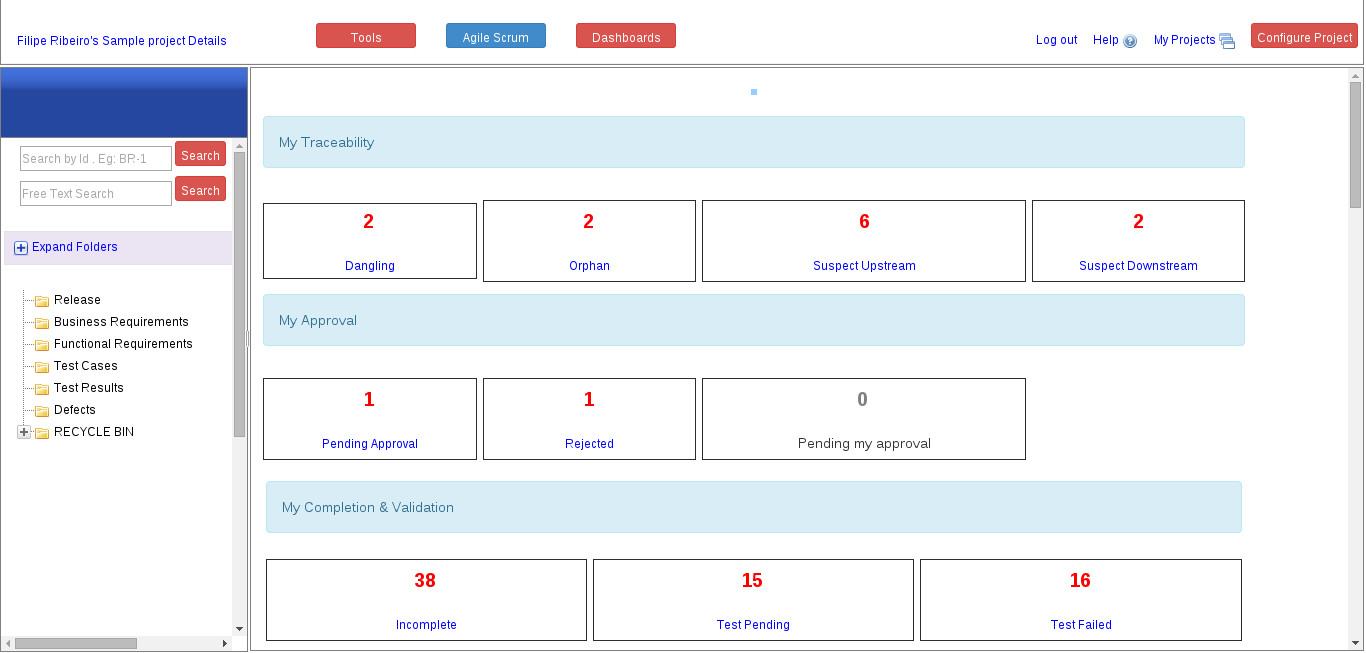
\includegraphics[scale=0.3]{figuras/trace.jpg}
\caption{Tela inicial da ferramenta TraceCloud}
\label{Rotulo}
\end{figure}

\subsection{Caliber}
A instalação da ferramenta é fácil, sendo necessário fazer um cadastro. A ferramenta é paga, mas possui a versão para testes por 30 dias.
Foi escolhida essa versão para avaliar a ferramenta.

A ferramenta gerencia muito bem os requisitos nos seguintes critérios:
\begin{itemize}
  \item Mudança dos requisitos;
  \item Prioridade dos requisitos;
  \item Rastreabilidade;
  \item Relacionamento dos requisitos;
  \item Análise dos requisitos.
\end{itemize}

Qualquer alteração que os requisitos sofrem é registrada pela ferramenta no histórico de mudanças a data e hora da mudança, o responsável e há
também a possibilidade de se fazer um comentário referente a tal mudança.

A organização dos itens da ferramenta usa um padrão já conhecido pelos usuários de outras ferramentas similares, barra a esquerda com os dados do projeto,
menu na barra superior. Isso torna a ferramenta fácil de usar, evitando que o usuário fique confuso.

\begin{figure}[!htb]
\centering
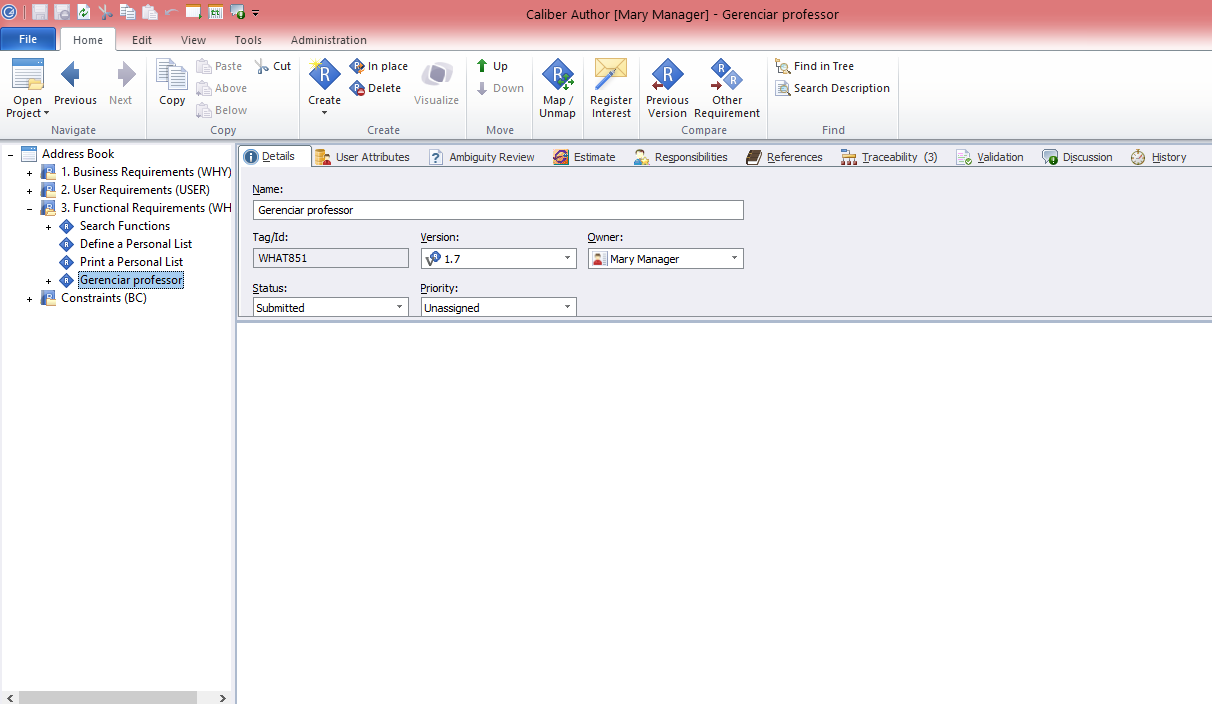
\includegraphics[scale=0.4]{figuras/caliber.png}
\caption{Tela inicial da ferramenta Caliber}
\end{figure}

\section[Escolha da Ferramenta]{Escolha da Ferramenta}
A ferramenta escolhida foi o TraceCloud. Como já dito, o TraceCloud é uma ferramenta \textit{web}, portanto o grupo se compromete e assume os riscos de conseguir apresentar as documentações geradas por ela independente da qualidade da internet em dias de apresentação. 
A vantagem é que todos componentes do grupo ganham uma maior autonomia com todos podendo alterar os documentos sempre que necessário, 
pois em casos de ferramentas offline, certamente seria necessário a delegação da função para um único aluno ficar responsável por gerenciar 
tais requisitos, o que é um grande risco, visto que o arquivo do computador pode sofrer um dano assim como o próprio sistema local.

Como explicado e avaliado na Figura \ref{fig:quadro}, as ferramentas avaliadas pelo grupo receberam notas de 0 a 5 em algumas características 
previamente estudadas, e comparando com as outras ferramentas avaliadas, em vários quesitos ela obteve a melhor pontuação. 
Em especial, no tópico que diz respeito ao processo de Engenharia de Requisitos da Empresa Junior de Engenharia de Energia, a ferramenta possui 
uma opção de escolha entre metodologias ágeis e tradicionais, sendo que cada uma recebe um melhor tratamento e as instruções que melhor se adequam 
ao trabalho. Além de fornecer um suporte ao SCRUM, tal ferramenta pode documentar as datas das modificações que os requisitos recebem ao longo do 
projeto garantindo total rastreabilidade dos mesmos e auxiliando na gerência de mudanças.

Por fim, outro ponto que se deseja utiizar bastante é o delegamento de funções por iteração. Tendo em vista que a cada período de tempo 
algumas tarefas deverão ser feitas, hora individuais e hora em grupo, para obtenção de um maior controle, organização e para reforço do 
cronograma (usado com outra ferramenta).

